% Drawing 74/07-4 -- folder 74, batch 07, archive page 125 (PDF page 126).
% Transcription: un hexagone orienté $z' \to x \to y' \to z \to x' \to y$, précédé d'une esquisse raturée ; à côté, des lignes $a - b - c \to a$ et leurs permutations, \uncertain{} pour la plupart.
% Kind: oriented hexagon; rows a - b - c. Method 2 (schematic redraw from the facsimile). Status: ok.
% Notes: The oriented hexagon z' -> x -> y' -> z -> x' -> y, drawn as arrows between the letters as on the page (the closing edge y -> z' is not visible and not drawn). Below, « (a, b, c) », and three rows of letters joined by strokes, the last stroke of each an arrow: a - b - c -> a, b - a - a -> c, c - c - b -> b (letters read on the facsimile; the transcription leaves most of them uncertain). Labels at \small. Struck out and omitted: the sketch x -> y' -> z before the hexagon (struck according to the transcription; on the facsimile it is the same chain begun once and given up), and the double stroke after « (a, b, c) », which is a strike-out, not an arrow. Redrawn 2026-11-09 (issue 128): to check again. Revised 2026-11-09 after Michel's check (#135): yes, as redrawn (the first sketch is struck); « there is no arrow next to (a, b, c) it's just struck »: the double arrow after (a, b, c) is removed.
% Coordinates: 1 unit = 1 mm = 1/100 of the crop width (bbox in page fractions: [0.4, 0.44, 0.95, 0.6]).
% Redrawn by Claude (claude-opus-5-5), issue #73, 2026-11-09; not checked by a human; not compiled (no TeX in the session).
% Revised by Claude (claude-opus-5-5) 2026-11-09 after Michel's check (#135): the double arrow after (a, b, c) removed (a strike-out); ok. Not compiled. Status: ok.
% Rights: reproduces part of the work -- behind RENDER_TRANSCRIPTS, never published by itself.
\documentclass[tikz,border=3pt]{standalone}
\usepackage{amsmath,amssymb}
\usetikzlibrary{patterns,arrows.meta}
\tikzset{pencil/.style={black!45}, struck/.style={black!35}, mark/.style={circle,draw,inner sep=1.3pt}, pt/.style={circle,fill,inner sep=0.9pt}, opt/.style={circle,draw,fill=white,inner sep=1.1pt}}
\begin{document}
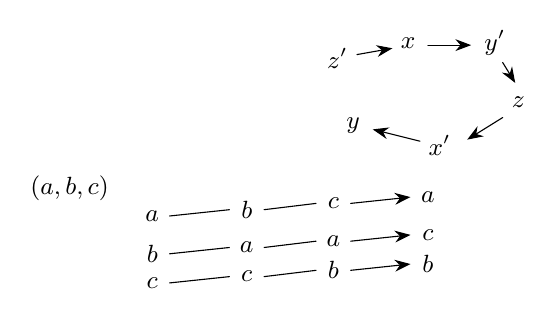
\begin{tikzpicture}[x=1mm,y=1mm,line cap=round,line join=round,font=\scriptsize]
\node[inner sep=1pt] at (55,-10.5) {\small $z'$};
\node[inner sep=1pt] at (64,-8.5) {\small $x$};
\node[inner sep=1pt] at (75,-8.5) {\small $y'$};
\node[inner sep=1pt] at (78,-16) {\small $z$};
\node[inner sep=1pt] at (68,-21.5) {\small $x'$};
\node[inner sep=1pt] at (57,-19) {\small $y$};
\draw[-{Stealth[length=2mm]}] (57.5,-10) -- (62,-9.2);
\draw[-{Stealth[length=2mm]}] (66.5,-8.8) -- (72,-8.8);
\draw[-{Stealth[length=2mm]}] (76,-11) -- (77.6,-13.6);
\draw[-{Stealth[length=2mm]}] (76,-18) -- (71.5,-20.8);
\draw[-{Stealth[length=2mm]}] (65.5,-21) -- (59.5,-19.5);
\node[inner sep=1pt] at (21,-27) {\small $(a,b,c)$};
\node[inner sep=1pt] at (31.5,-30.5) {\small $a$};
\node[inner sep=1pt] at (43.5,-29.7) {\small $b$};
\node[inner sep=1pt] at (54.5,-28.9) {\small $c$};
\node[inner sep=1pt] at (66.5,-28.1) {\small $a$};
\draw (33.7,-30.5) -- (41.3,-29.7);
\draw (45.7,-29.7) -- (52.3,-28.9);
\draw[-{Stealth[length=2mm]}] (56.7,-28.9) -- (64.3,-28.1);
\node[inner sep=1pt] at (31.5,-35.3) {\small $b$};
\node[inner sep=1pt] at (43.5,-34.5) {\small $a$};
\node[inner sep=1pt] at (54.5,-33.7) {\small $a$};
\node[inner sep=1pt] at (66.5,-32.9) {\small $c$};
\draw (33.7,-35.3) -- (41.3,-34.5);
\draw (45.7,-34.5) -- (52.3,-33.7);
\draw[-{Stealth[length=2mm]}] (56.7,-33.7) -- (64.3,-32.9);
\node[inner sep=1pt] at (31.5,-39) {\small $c$};
\node[inner sep=1pt] at (43.5,-38.2) {\small $c$};
\node[inner sep=1pt] at (54.5,-37.4) {\small $b$};
\node[inner sep=1pt] at (66.5,-36.6) {\small $b$};
\draw (33.7,-39) -- (41.3,-38.2);
\draw (45.7,-38.2) -- (52.3,-37.4);
\draw[-{Stealth[length=2mm]}] (56.7,-37.4) -- (64.3,-36.6);
\end{tikzpicture}
\end{document}
